\documentclass[a4paper,12pt]{article}
\pdfoutput=1 % if your are submitting a pdflatex (i.e. if you have
             % images in pdf, png or jpg format)

\usepackage{jheppub} % for details on the use of the package, please
                     % see the JHEP-author-manual
\usepackage[T1]{fontenc} % if needed
\usepackage{float}
\usepackage{cancel}
%\graphicspath{{../calcs/}}

%\title{\boldmath A title with some math: $x=1$}
\title{CP Violation In and Beyond The Standard Model: Two Higgs Doublet Model Corrections to Standard Model Flavour Observables}


%% %simple case: 2 authors, same institution
%% \author{A. Uthor}
%% \author{and A. Nother Author}
%% \affiliation{Institution,\\Address, Country}

% more complex case: 4 authors, 3 institutions, 2 footn#otes
\author{Matthew Rossetter}

% The "\note" macro will give a warning: "Ignoring empty anchor..."
% you can safely ignore it.

\affiliation{Supervised By Alexander Lenz}
\affiliation{MPhys Theoretical Physics, Durham University}

% e-mail addresses: one for each author, in the same order as the authors
%\emailAdd{matthew.rossetter@durham.ac.uk}

\abstract{Abstract...}

\begin{document} 
\maketitle
\flushbottom

\section{Introduction}
The Standard Model is one of the most successful theories ever developed, describing the fundamental forces currently observed, excluding gravity, through a quantum field theory Lagrangian, see \eqref{eq:sm}.
Throughout the latter half of the 20th century and through the 21st, the Standard Model has found strong agreement with many observed phenomena, while also predicting many other observables that were took longer to be observed (most notably, the Higgs boson).
\begin{equation}
    \label{eq:sm}
    \begin{split}
        \mathcal{L} = -&\frac14 F^{\mu\nu}F_{\mu\nu} \qquad\qquad\qquad\quad\to \text{gauge term}\\
                      +& i\bar{\psi}\cancel{D}\psi \qquad\qquad\qquad\qquad\;\to \text{Fermion term} \\
                      +& (D_\mu\phi)^\dagger(D^\mu\phi) - V(\phi) \quad\;\;\,\to \text{Higgs term}\\
                      -& Y_{ij}\bar{\psi}_i\phi\psi_j + h.c. \qquad\qquad\;\to\text{Yukawa term}
    \end{split}
\end{equation}
However, there are still many observations that do not align with the Standard Model; some more large scale such as unification with gravity or a description of dark matter, some more specific such as B meson oscillation frequencies or leptonic and semi-leptonic meson decays.
The smaller scale innacuracies may seem less important than the larger scale ones, but the modifications to the Standard Model required to realign these observables open the door to possibilities for new physics models, perhaps with new particles and new forces at play.

\subsection{The Standard Model}
The physics of the Standard Model is perfectly contained within its Lagrangian in \eqref{eq:sm}, and most of its terms can be expanded to more clearly describe each part of the theory. 
This theory is a quantum field theory so all particles of the theory are quantum fields permeating throughout space time. 
There are twenty-five fundamental particles currently described in the Standard Model: twelve fermions (quarks and leptons), four gauge bosons of the electroweak theory ($W^\pm,Z,\gamma$), eight gluons of the strong force, and the Higgs boson.

The basis for the Standard Model are the quantum theories of electroweak and strong interactions, and then the symmetry breaking Higgs mechanism to give masses to these theories.
Both the electroweak and strong theories are non-Abelian gauge theories of massless fermions; the electroweak theory has a gauge symmetry of SU(2)$_{L}\otimes$U(1), and strong of SU(3)$_{c}$.
To formulate the Standard Model Lagrangian, we start with the free Lagrangian of a massless Dirac fermion coupled to a gauge field tensor,
\begin{equation}
    \label{eq:dirac}
    \mathcal{L} = i\bar{\psi}\gamma^\mu\partial_\mu\psi - \frac14F^{\mu\nu}F_{\mu\nu}
\end{equation}
\begin{itemize}
    \item impose gauge transformation
    \item $\partial\to D$
    \item Tr and $f^{abc}$
    \item Weak imposes lefthandedness
    \item SSB and Higgs, Yukawa
    \item Combine for SM
\end{itemize}

\subsection{Flavour Observables and Inconsistencies}
\begin{itemize}
    \item Sakharov criteria? -> CPv needed
    \item Exp vs Theory no agree, diagram
    \item Indicates searching for new physics
    \item New Z', 2HDM, SM4, etc
    \item Any new theory must be renormalisable, and also be consistent in modifying SM - can't fix some problems while sacrificing other results
\end{itemize}

\subsection{2HDM Explanation}
\begin{itemize}
    \item Add second doublet instead of h.c.
    \item Two VEVs, 5 bosons
    \item Adjustment to theory
\end{itemize}

\section{Testing of 2HDM}
\begin{itemize}
    \item Follow lots from 0907.5135
    \item Explain each type of observable
    \item Input parameters
\end{itemize}
\begin{figure}[H]
    \centering
    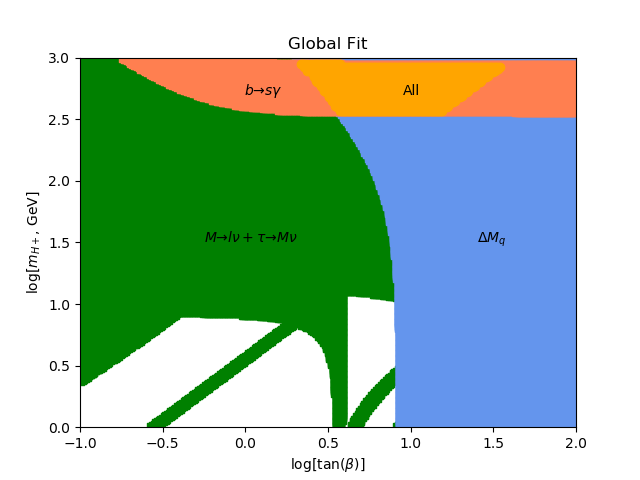
\includegraphics[scale=0.8]{../calcs/global.png}
    \caption{\label{fig:glob} Global fit, tadaaaaa}
\end{figure}

\section{Next?}

\appendix
\section{Some title}
Please always give a title also for appendices.

\acknowledgments
This is the most common positions for acknowledgments. A macro is
available to maintain the same layout and spelling of the heading.

\paragraph{Note added.} This is also a good position for notes added
after the paper has been written.





% The bibliography will probably be heavily edited during typesetting.
% We'll parse it and, using the arxiv number or the journal data, will
% query inspire, trying to verify the data (this will probalby spot
% eventual typos) and retrive the document DOI and eventual errata.
% We however suggest to always provide author, title and journal data:
% in short all the informations that clearly identify a document.

%\section{Some examples and best-practices}
%\label{sec:examples}
%
%For internal references use label-refs: see section~\ref{sec:examples}.
%Bibliographic citations can be done with cite: refs.~\cite{a,b,c}.
%When possible, align equations on the equal sign. The package
%\texttt{amsmath} is already loaded. See \eqref{eq:x}.
%\begin{equation}
%\label{eq:x}
%\begin{split}
%x &= 1 \,,
%\qquad
%y = 2 \,,
%\\
%z &= 3 \,.
%\end{split}
%\end{equation}
%Also, watch out for the punctuation at the end of the equations.
%
%The amsmath package has many features. For example, you can use use\\
%\texttt{subequations} environment:
%\begin{subequations}\label{eq:y}
%\begin{align}
%\label{eq:y:1}
%a & = 1
%\\
%\label{eq:y:2}
%b & = 2
%\end{align}
%and it will continue to operate across the text also.
%\begin{equation}
%\label{eq:y:3}
%c = 3
%\end{equation}
%\end{subequations}
%The references will work as you'd expect: \eqref{eq:y:1},
%\eqref{eq:y:2} and \eqref{eq:y:3} are all part of \eqref{eq:y}.
%
%A similar solution is available for figures via the \texttt{subfigure}
%package (not loaded by default and not shown here). 
%All figures and tables should be referenced in the text and should be
%placed at the top of the page where they are first cited or in
%subsequent pages. Positioning them in the source file
%after the paragraph where you first reference them usually yield good
%results. See figure~\ref{fig:i} and table~\ref{tab:i}.
%
%\begin{figure}[tbp]
%\centering % \begin{center}/\end{center} takes some additional vertical space
%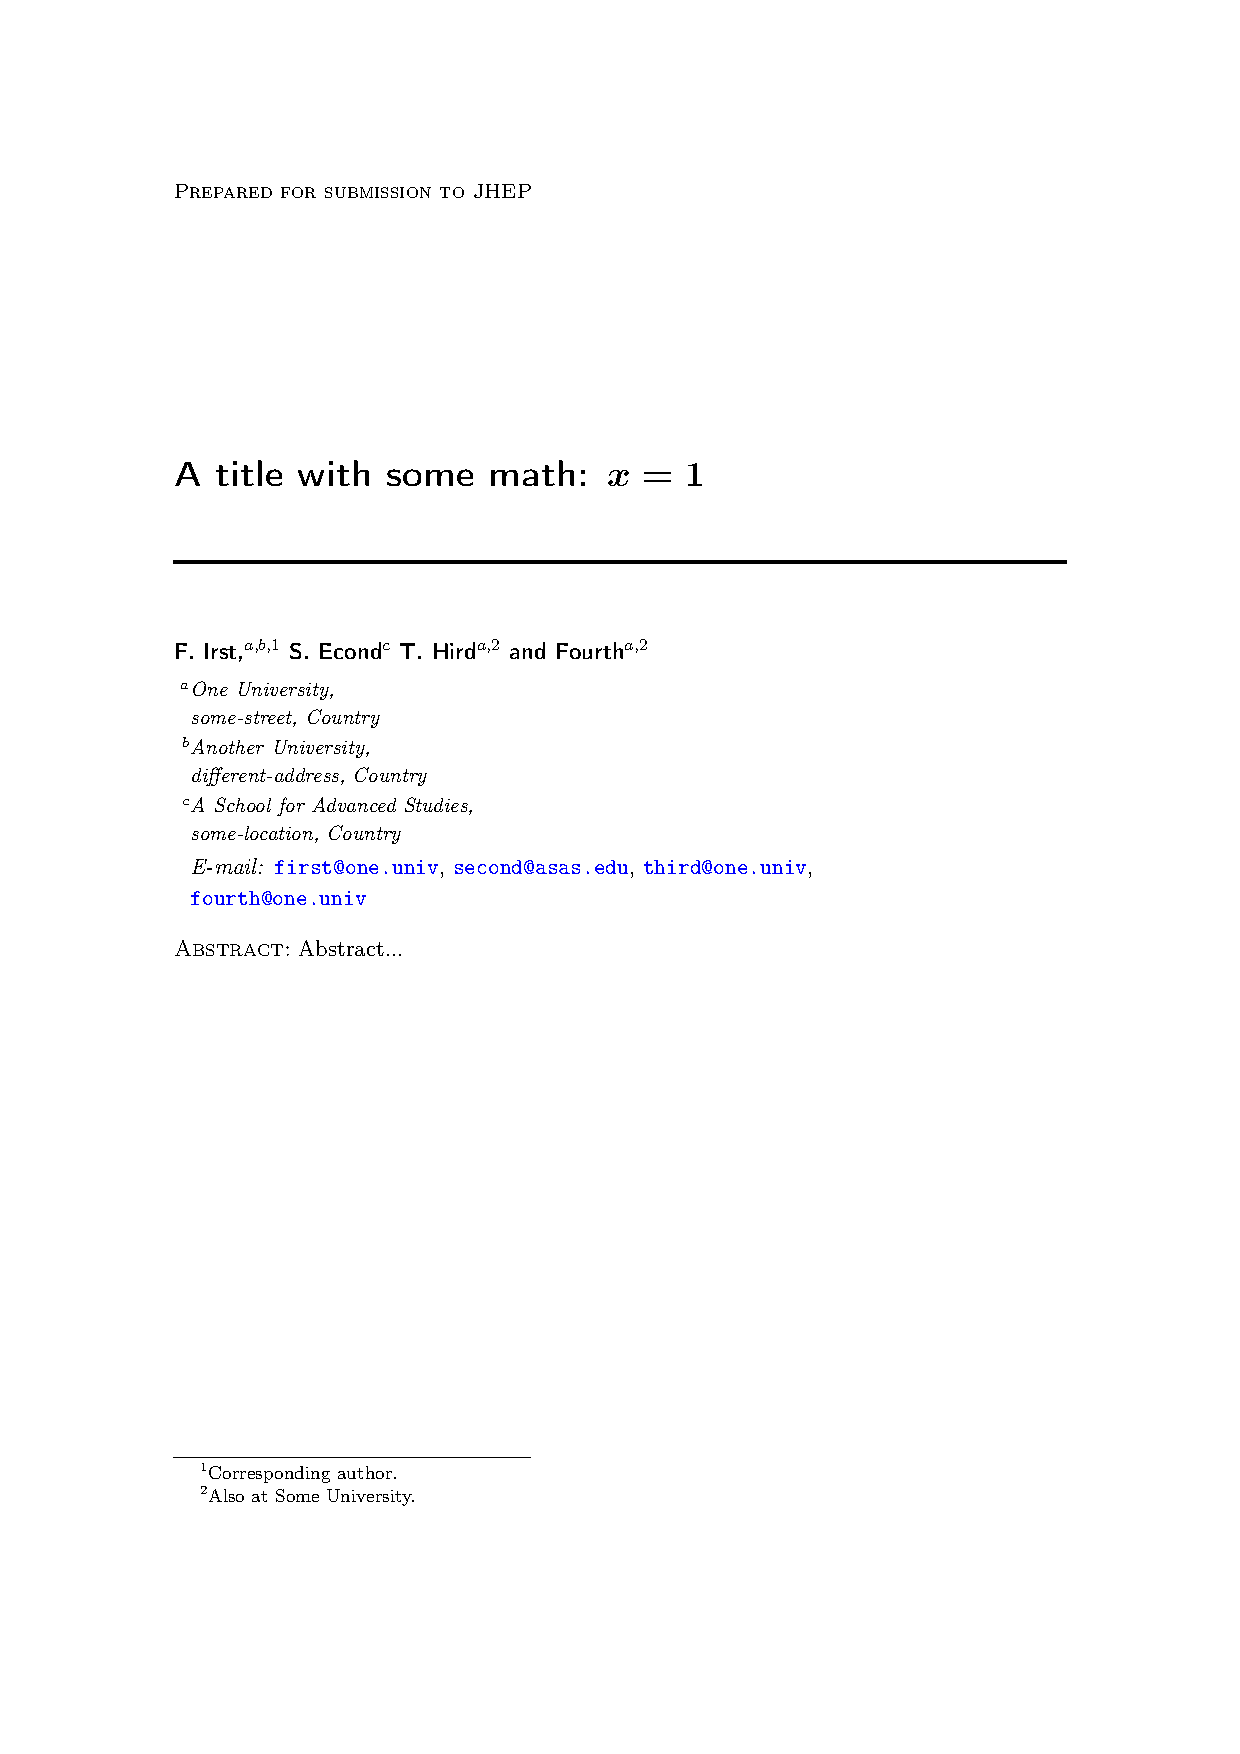
\includegraphics[width=.45\textwidth,trim=0 380 0 200,clip]{img1.pdf}
%\hfill
%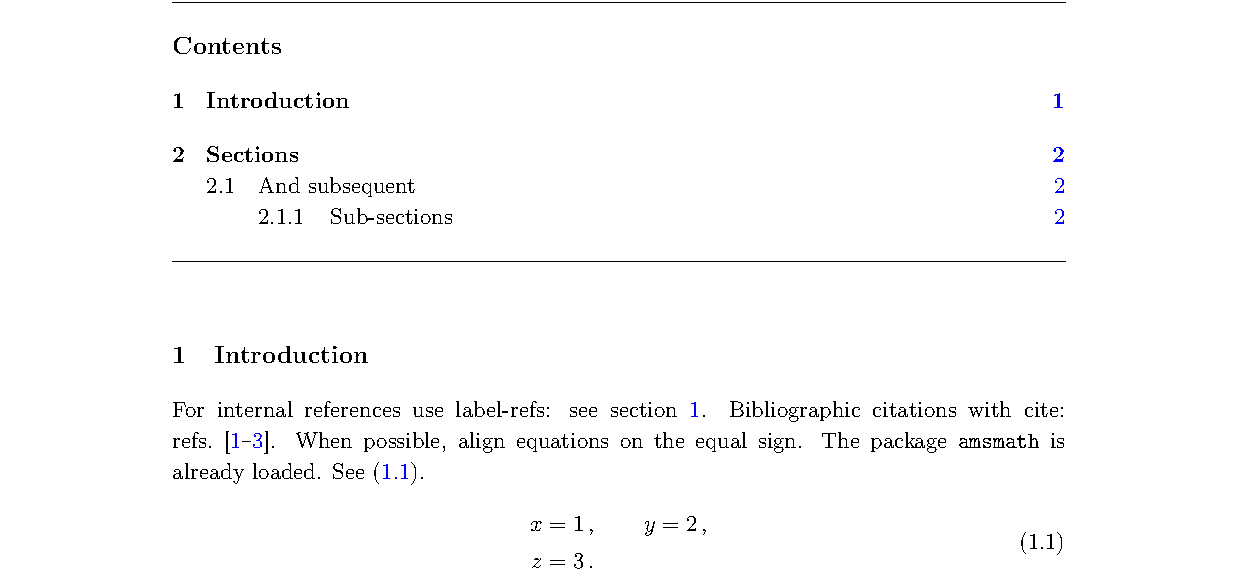
\includegraphics[width=.45\textwidth,origin=c,angle=180]{img2.pdf}
%% "\includegraphics" is very powerful; the graphicx package is already loaded
%\caption{\label{fig:i} Always give a caption.}
%\end{figure}
%
%\begin{table}[tbp]
%\centering
%\begin{tabular}{|lr|c|}
%\hline
%x&y&x and y\\
%\hline 
%a & b & a and b\\
%1 & 2 & 1 and 2\\
%$\alpha$ & $\beta$ & $\alpha$ and $\beta$\\
%\hline
%\end{tabular}
%\caption{\label{tab:i} We prefer to have borders around the tables.}
%\end{table}
%
%We discourage the use of inline figures (wrapfigure), as they may be
%difficult to position if the page layout changes.
%
%We suggest not to abbreviate: ``section'', ``appendix'', ``figure''
%and ``table'', but ``eq.'' and ``ref.'' are welcome. Also, please do
%not use \texttt{\textbackslash emph} or \texttt{\textbackslash it} for
%latin abbreviaitons: i.e., et al., e.g., vs., etc.
%
%\paragraph{Up to paragraphs.} We find that having more levels usually
%reduces the clarity of the article. Also, we strongly discourage the
%use of non-numbered sections (e.g.~\texttt{\textbackslash
%  subsubsection*}).  Please also see the use of
%``\texttt{\textbackslash texorpdfstring\{\}\{\}}'' to avoid warnings
%from the hyperref package when you have math in the section titles


\begin{thebibliography}{99}

\bibitem{a}
O. Deschamps et al, \emph{The Two Higgs Doublet Model of Type II facing flavour physics data}, \href{https://arxiv.org/pdf/0907.5135.pdf}{arxiv:0907.5135}.

\bibitem{b}
G. Degrassi, P. Gambino, and P. Slavich, \emph{SusyBSG: a fortran code for BR$[\to X_s\gamma]$ in the MSSM with Minimal Flavor Violation}, \href{https://arxiv.org/pdf/0712.3265.pdf}{arxiv:0712.3265}.

\bibitem{c}
Y. Amhis et al [HFLAV], \emph{Averages of b-hadron, c-hadron, and $\tau$-lepton properties as of 2018}, \href{https://arxiv.org/pdf/1909.12524.pdf}{arxiv:1909.12524}.

\bibitem{d}
M. Tanabashi et al [Particle Data Group], Phys. Rev. D98, 030001 (2018) and 2019 update

\bibitem{e}
A. Sibidanov et al [Belle], \emph{Study of Exclusive $B\to X_ul\nu$ Decays and Extraction of $|V_{ub}|$ using Full Reconstruction Tagging at the Belle Experiment}, \href{https://arxiv.org/pdf/1306.2781.pdf}{arxiv:1306.2781}.

\bibitem{f}
A. Lenz and G. Tetlalmatzi-Xolocotzi, \emph{Model-independent bounds on new physics effects in non-leptonic tree-level decays of B-mesons}, \href{https://arxiv.org/pdf/1912.07621.pdf}{arxiv:1912.07621}.


% Please avoid comments such as "For a review'', "For some examples",
% "and references therein" or move them in the text. In general,
% please leave only references in the bibliography and move all
% accessory text in footnotes.

% Also, please have only one work for each \bibitem.


\end{thebibliography}
\end{document}
